\subsubsection{Graptemys --- Map Turtles}
\begin{center}
\begin{longtabu} to \textwidth {| | p{3.5cm} | X | |}

	\hline
	Taxonomy/Ancestry &
	13 species. also known as ``sawback turtles." Member of subfamily Deirochelyinae.
	
	\begin{center} 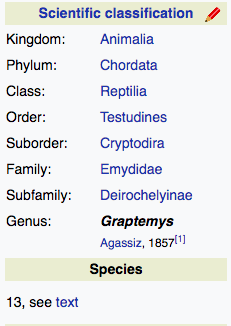
\includegraphics[scale=0.5]{testudines/emydidae/graptemys/tax} \end{center}
	 \\
	\hline
	Size & 
	Males: 3-7 in
	
	Females: 7-10 in
	\\
	\hline
	Color &
	the lines on the shell resemble waterways on maps. it has thicker, yellow lines on the limbs and face.
	 \\
	\hline
	Anatomy &
	resemble many other aquatic turtles, but distinguished by keel running length of center of carapace. some have spike-like juts along the keel. live 15-100 years.
	 \\
	\hline
	Dimorphism & 
	females larger than males. 
	
	males have much longer claws on the front legs.
	
	Females can be partitioned into 3 groups based on head width/amt of mollusks eaten --- Microcephalic (narrow, consume few mollusks); Mesocephalic (wider, mostly mollusks w/ softer-bodied prey); Megacephalic (widest, almost entirely mollusks) 
	\\
	\hline
	Behavior & 
	spend many hours basking. they are communal w/ other turtles --- share space and use each other for predator-watching.
	\\
	\hline
	Habitat & 
	\begin{itemize}[noitemsep]
		\item mostly aquatic, but spend some time on land
		\item live only in freshwater, like ponds/rivers, and prefer flowing water
		\item ideal environment = underwater plant matter to eat; rocks and logs to bask on
	\end{itemize}
	\\
	\hline
	Distribution & 
	found throughout eastern half of US and northwards into southern Canada
	\\
	\hline
	Feeding Ecology & 
	\begin{itemize}[noitemsep]
		\item more carnivorous than most Emydids
		\item females have wider heads --- eat mollusks, insects, crayfish
		\item males w/ smaller heads --- smaller mollusks and insects
		\item feeding is always in the water
	\end{itemize}
	\\
	\hline
	Reproductive Biology & 
	\begin{itemize}[noitemsep]
		\item breed in spring/fall
		\item mating takes place in deep waters
		\item nesting period in May-July
		\item prefer unshaded sites of sandy soil
		\item usually lay 2 or more clutches of 6-20 eggs
		\item hatch after 50-70 days in August-September
		\item may overwinter in nest
		\item TSD
			\begin{itemize}[noitemsep]
				\item $25^\circ$C = male
				\item 30-35$^\circ$C = female
			\end{itemize}
	\end{itemize}
	\\
	\hline
	Ecological Role &
	control invasive mollusks like zebra mussels and Asian clams
	\\
	\hline
	Conservation Status & 
	5 LC; 3 EN; 2 VU; 2 NT
	
	3 species bred heavily for pet trade in 1970s but slowly decreased in popularity
	\\
	\hline
\end{longtabu}
 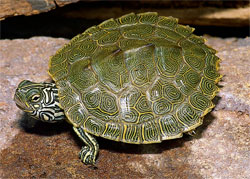
\includegraphics[scale=0.75]{testudines/emydidae/graptemys/1} 
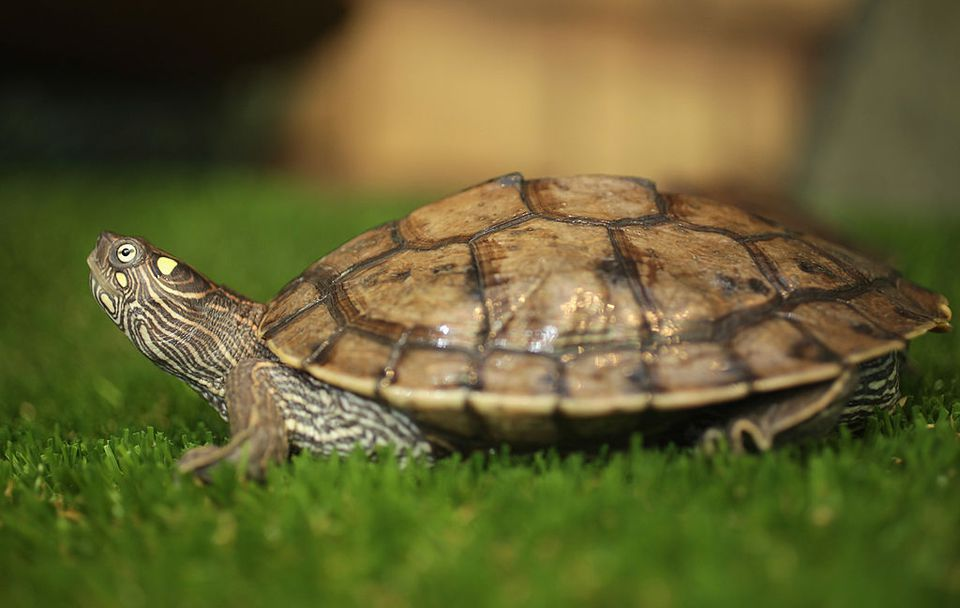
\includegraphics[scale=0.2]{testudines/emydidae/graptemys/2}
\end{center}